\documentclass[11pt, a4paper]{report}
\usepackage[utf8]{inputenc}
\usepackage{float}
\usepackage{array}
\usepackage{amsmath}
\usepackage{amssymb}
\usepackage{amsfonts}
\usepackage{latexsym}
\usepackage{graphicx}
\usepackage{tabularx}
\usepackage{ltxtable}
\usepackage{longtable}
\usepackage{color, colortbl}
\usepackage{caption}
\usepackage{ifpdf}
\usepackage[hidelinks]{hyperref}
\usepackage{url}
\usepackage{xtab}
\usepackage[hmargin=3cm,vmargin=3cm]{geometry}
\usepackage[norsk, english]{babel} 
\usepackage[parfill]{parskip}
\usepackage{pdfpages}


% Begin chapter numbering
\usepackage[T1]{fontenc}
\usepackage{titlesec, blindtext, color}

\definecolor{gray75}{gray}{0.75}
\newcommand{\hsp}{\hspace{20pt}}
\titleformat{\chapter}[hang]{\Huge\bfseries}{\thechapter\hsp\textcolor{gray75}{|}\hsp}{0pt}{\Huge\bfseries}
% End chapter numbering

% Add numbering to subsubsection
\setcounter{secnumdepth}{3}
\setcounter{tocdepth}{3}

%\newcommand{\newCommandName}{text to insert} % Defines a variable in LaTeX
\newcommand{\comment}[1]{} \comment{This is a block comment wrapped in curly brackets}
%\renewcommand{\thefootnote}{\roman{footnote}}

\definecolor{Gray}{gray}{0.9}


\begin{document}
\pagenumbering{gobble}

\begin{titlepage}
\begin{center}
\vspace*{1in}
{\LARGE IT2901 - Informatikk prosjektarbeid II}
\par
\vspace{1cm}


\begin{figure}[ht!]
\centering

\includegraphics[width=25mm]{images/ic_launcher.png}
%\caption{A simple caption}
\label{overflow}
\end{figure}


{\LARGE $\mu$C Software Store}
\par
\vspace{0.6in}
{\LARGE Project Report}
\par
\vspace{0.2in}
{\Large 09\_Arduino}
\par
\vfill
\par
\vspace{0.5in}
Jeppe Eriksen, Bjørn Arve Fossum, Ståle Semb Hauknes,\\ Wilhelm Walberg Schive, Nina Margrethe Smørsgård, Robin Tordly\\
\par
%\today %Month Year -formatting?
\end{center}
\end{titlepage}

\newpage

\tableofcontents
\newpage
\pagenumbering{arabic}
\section{Introduction}
\subsection{The group}
The group consisted of six students from Computer Science at NTNU, each possessing different technical skills.

%TODO: fix bullet list NINA!!
\item{\Wilhelm Walberg Schive}\newline %er detta riktig?
	Third year Informatics student at NTNU. Experience with Java, MySQL and knew the basics of Arduino project development.


\subsection{Problem description}
The project task was to develop a platform for easy use, setup and sharing of Physical User Interfaces (PUIs) for Arduino. The task was divided in three main parts: a market application, over the air installation and example PUIs.\\
\newline
The purpose of the market application was to allow users of Arduino to browse and download PUI applications for their Arduino board on a mobile Android device. This market app was to be a simplified version of e.g. Google Play, where users easily can browse and install whatever applications they desire. An application selected for installation in the market application should be prepared on the mobile device, and installed over the air on an Arduino board using Bluetooth. The example PUIs were mostly intended to demonstrate the feasibility of the finished product.

\subsection{The goal}
The goal of the project task was to make Arduino easier to use for ordinary people, by allowing easy browsing, sharing and installation of applications on Arduino boards. By developing an application for over the air installation of applications, the finished product should ease the process of both installing and updating PUIs on an Arduino.

\section{Definitions}
This is a list of terms and abbreviations used throughout the project report in order to clarify and explain their meaning.

\begin{description}

\item[Android:]
An operating system for mobile devices based on the Linux operating system. It is developed by Google and the Open Handset Alliance. Applications for Android devices are written in Java, and all the software is open source released under the Apache License.

\item[Apache:]
A software foundation focused on open source and community driven software.

\item[Arduino:]
A tool for making Physical User Interfaces (PUIs). It is an open-source physical computin platform based on a simple microcontroller board.

\item[PUI:]
An acronym for Physical User Interface. A PUI is a user interface which interacts with digital information through the physical environment. 


\subsection{Work breakdown structure (WBS)}
The WBS is a view on what work packages the project encompasses. It helps with communicating the work and processes to easily execute the project. The duration-time show how much estimated time one task require, and gives an assessment on how much effort to be considered.\\
\newline
\textbf{The Dictionary View} is an organized table view of the WBS with a simple structure. The Duration column is an extension of the original Dictionary View.\\

\begin{longtable}{|m{0.1 \textwidth}|m{0.1 \textwidth}|m{0.2 \textwidth}|m{0.35\textwidth}|m{0.15 \textwidth}|}
\hline
	\rowcolor{Gray}
	\textbf{Level} & \textbf{WBS{ }Code} & \textbf{Element name} & \textbf{Definition} & \textbf{Duration}\\
	\endfirsthead% 
	\multicolumn{5}{l}%
	{{\bfseries Continued from previous page}} \\ \hline
	\rowcolor{Gray}
	\textbf{Level} & \textbf{WBS{ }Code} & \textbf{Element name} & \textbf{Definition} & \textbf{Duration}\\
\hline
	\endhead%
	\hline
 
	\hline \multicolumn{5}{|l|}{{Continued on next page}} \\ \hline
	\endfoot%
 
	\endlastfoot%

	1 & 1 & $\mu$C Software Store & All work to implement an application store for Arduinos and over the air innstallation with two example PUIs & \\
\hline
	2 & 1.1 & Project management & The work to initiate the project and distribute responsibilities & \\
\hline
	3 & 1.1.1 & Meetings with customer & Determine the project status and decide on requirements & \\
	 & 1.1.2 & Demonstration and play for the customer of the team's understanding of the requirements & Project team evaluates and proposes recommendations & \\
\hline
	 & 1.1.3 & Risk management & Creating risk analysis and agreements within the group and the project & \\
\hline
	 & 1.1.4 & Status report & Write the status report & \\
\hline
	2 & 1.2 & Planning & & \\
\hline
	3 & 1.2.1 & Requirements specification & & \\
\hline
	 & 1.2.2 & Determine Project team & Give each menber a role and distribute tasks & \\
\hline
	 & 1.2.3 & Supervisor meeting & Meeting wih supervisor for instruction and guidance & \\
\hline
	 & 1.2.4 & Develop project plan and use cases & & \\
\hline
	 & 1.2.5 & Research & & \\
\hline
	 & 1.2.5.1 & Research on over the air innstallation & Do research on bluetooth installation on arduinos & \\
\hline
	 & 1.2.5.2 & Research UbiCollab libraries & & \\
\hline
	2 & 1.3 & Execution & Programming and execution of the project & \\
\hline
	3 & 1.3.1 & Project kickoff meeting & First meeting with customer to evaluate knowledge and agree on further meetings & \\
\hline
	 & 1.3.2 & Verify \& validate user requirements & Determine whether the group is in tune with the customers vision of the project requirements & \\
\hline
	 & 1.3.3 & Design system & & \\
\hline	  
	 & 1.3.4 & & & \\
\hline
	 & 1.3.5 & Produce Software & & \\
\hline
	 & 1.3.6 & Instalation over the air implementation & & \\
\hline
	 & 1.3.7 & Documentation & & \\
\hline
	2 & 1.4 & Testing & & \\
\hline
	3 & 1.4.1 & Develop unit tests & & \\
\hline
	 & 1.4.2 & User testing & & \\
\hline
	 & 1.4.3 & Stress testing & & \\
\hline
	 & 1.4.4 & System Testing & & \\
\hline
	2 & 1.5 & Closeout & & \\
\hline
	3 & 1.5.1 & Creating final project report & & \\
\hline
	 & 1.5.2 & Delivery to customer & & \\
\hline
\end{longtable}
\captionof{table}{Work Breakdown Structure}


\textbf{The Tree Structure}, which is the most popular WBS format, presents an easy to understand view into the WBS. The Tree Structure is not easy to make and is created with a tool: Microsoft Word and SmartArt graphics.\\
\begin{figure}[H]
\includegraphics[scale=0.7]{figures/wbstree.pdf}
\captionof{figure}{WBS Tree}
\end{figure}
\section{Prestudy}
\subsection{Development methods}
\subsubsection{Scrum}
Scrum is an iterative and incremental development framework for development of complex information systems. The use of Scrum requires the team to be divided into specific roles, where each role has its own responsibility. The following is the core roles of the Scrum team:
\begin{description}
	\item[Product owner:]{The product owner represents the stakeholders in the project, and is the voice of the customer. It is the product owner’s responsibility to ensure that the Scrum team at all times is working with the right things seen from a business perspective.}
	\item[Scrum master:]{The scrum master should act as a buffer between the development team and distracting influences, so that the development team can deliver potentially shippable products at the end of each sprint. The scrum master should keep the development team focused at all times.}
	\item[Development team:]{The development team is made up from three to nine persons with cross-functional skills. This team does the all the actual work, including development, testing, designing and so on.}
\end{description}

\subsubsection{Spiral model}
The spiral model is software development model intended for large and complicated projects. It combines elements from the waterfall model and prototyping models, and uses an iterative approach. Based on this it allows for incremental releases of the product.

\subsubsection{Lean sotfware development}
Lean is an agile software development methodology that is defined by seven principles:
\begin{description}
	\item[Eliminate waste.]{Everything that does not add any value to the customer is considered a waste.}
	\item[Amplify learning Defects.]{Should be prevented by running early after the code is made.}
	\item[Decide as late as possible.]{Better result should be achieved with an option-based approach. Delaying options as much as possible would give more flexibility later.}
	\item[Deliver as fast as possible.]{The sooner the product is delivered, the sooner feedback can be received.}
	\item[Empower the team.]{The managers are taught how to listen to the developers, so they can explain better what action that might be taken, and give suggestion for improvement.}
	\item[Build integrity.]{The customer needs to have more influence and inspection of the project.}
	\item[See the whole.]{Decompose the system into smaller parts and find and eliminate defects.}
\end{description}

\subsection{Existing solutions}
This is a summary of existing solutions similar to the project assignment. This section is divided in two subsections; one for the market application and one for the over-the-air transfer. The existing products were evaluated on the following criteria:
\begin{itemize}
	\item{To what degree the product fits the assignment.}
	\item{Can the product, or parts of it, be reused for the assignment? Can it lead to licensing issues?}
\end{itemize}

\subsubsection{Market application}
A prior project created an universal app store in PHP. Had potential for serving as a back end.

{\bf Google Play} is a similar market application for android that categorizes the applications and have a search option. It also detects what model of phone that is being used, and only shows apps that are supported by that phone. The applications are shown in lists and can be downloaded by two clicks. The first click guides you to a description section with pictures, description, comments and user-feedback in form of 5-star-rating.\\
The store is not open source and can only be a source of inspiration for this project.
\begin{figure}[H]
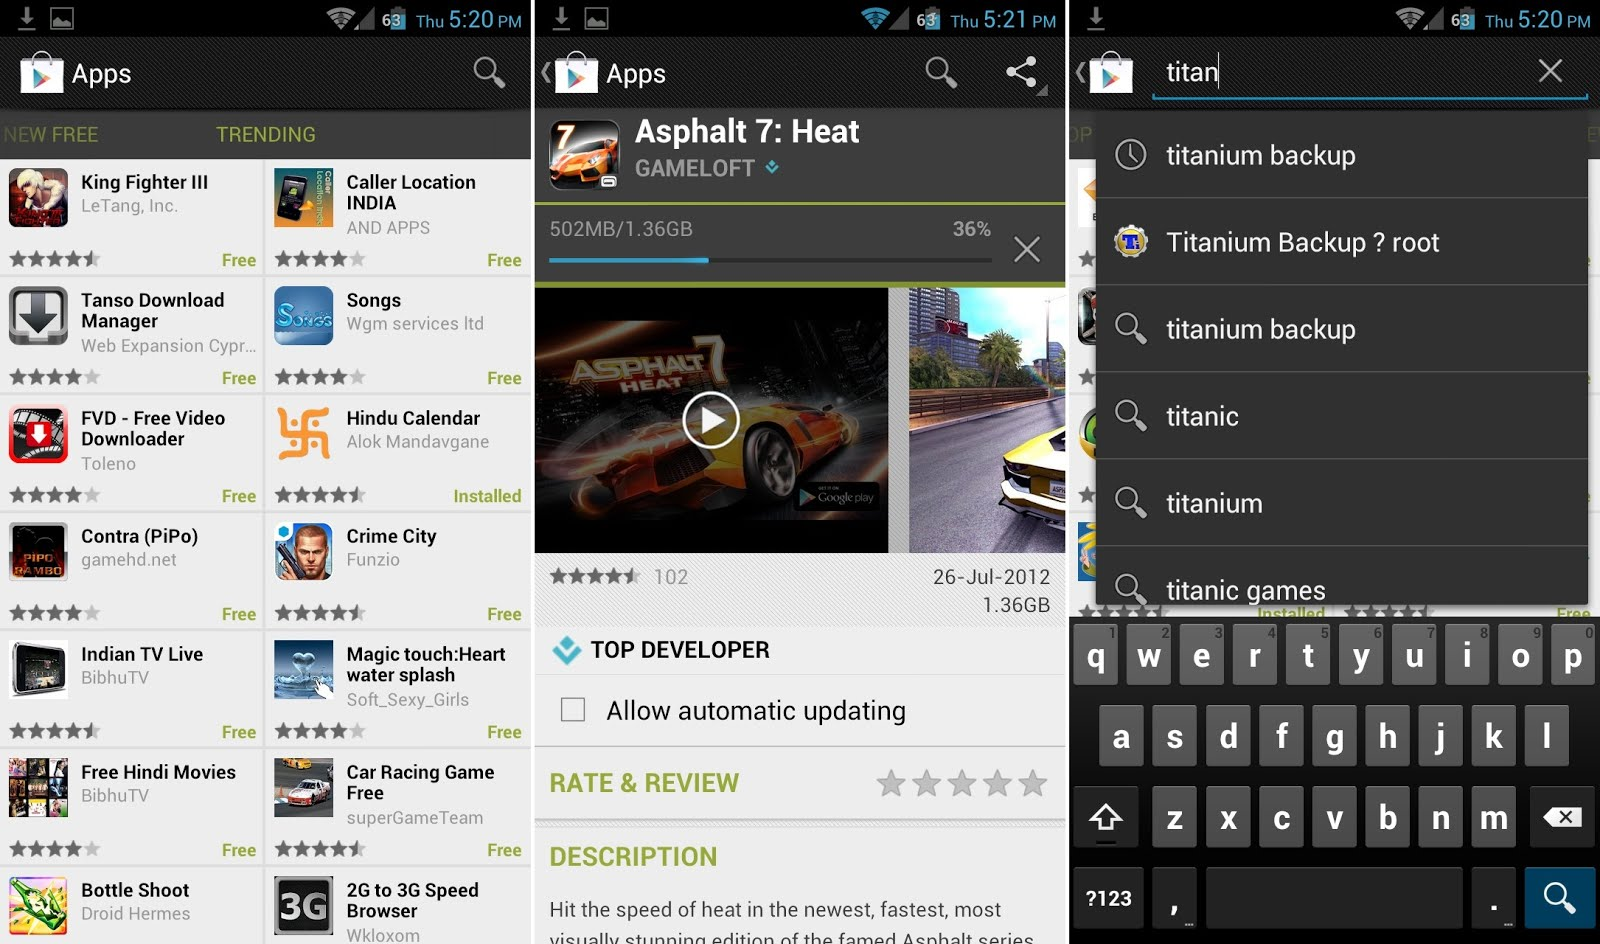
\includegraphics[scale=0.2]{images/Google-Play-Store-APK-3-7-15.jpg}
\caption{Google Play Store}
\end{figure}

{\bf App Store} is also a similar market application, but for apple products\ldots etc\ldots\\
\begin{figure}[H]
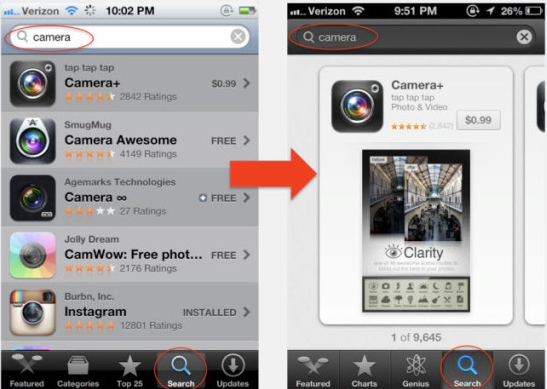
\includegraphics[scale=0.7]{images/png;base642dee0c596030bc1e.png}
\caption{App Store}
\end{figure}
These applications fit the assignment in the way that they are both market applications where one can download applications. This was useful for the development of the product, since it was possible to use the same principles in the assignment. It was also similar in the way that it was possible to browse for applications on the computer, and ''push'' the app to a mobile telephone. This, however, did not connect via bluetooth which the task assignment stated that the finished product should. Based on this, it was not possible to reuse the code or other parts of any of the applications in the development. 

\subsubsection{Over the air transfer}
Pebble is a watch that offers over the air transfer of applications. It is based on the same microchip as one of the newest Arduino\#, but contains an operating system written in C.
\begin{figure}[H]
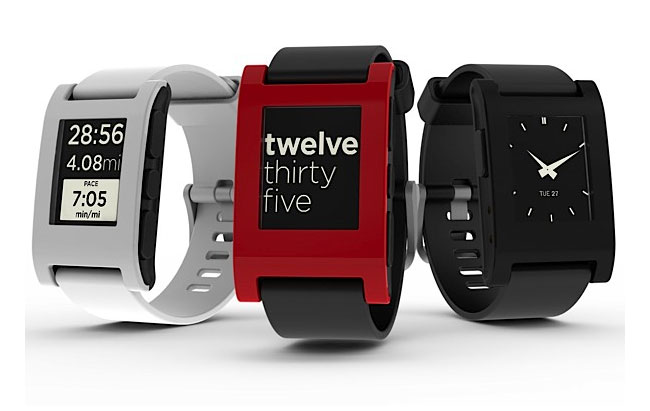
\includegraphics[scale=0.7]{images/Pebble-Smartphone-Watch.jpeg}
\caption{Pebble Watch}
\end{figure}
There was very little documentation on the Pebble website, so the potential reuse in this project appears minimal.
\chapter{Project Management}
The following sections details the project management decisions of the project. This includes choice of development method, team member responsibilities, communication channels and risk analysis.

\section{Development method}
Based on the customer requirement of short iterations, it was early decided to adapt an iterative and incremental development method for the project. By working in an iterative manner, it was possible to present prototypes and work done to the customer every week, and at the same time receive feedback. In this fashion it was possible for the customer to continuously present his thoughts on the product, and propose changes where he thought is was necessary. The iterative approach on the project also made it easier for the group to set deadlines and milestones of specific parts of the product.\\
\newline
All the members of the group have taken the course TDT4140 - Systemutvikling, and therefore have some knowledge about different development methods. The Rational Unified Process (RUP) model is an extensible framework\cite{kruchten} and was chosen for the project.

\subsection{Rational Unified Process}
Rational Unified Process (RUP) is an iterative and incremental software development process model. It is a process model that aims to capture the best practises in modern software development and present them in a tailorable form.\cite{kruchten} Each iteration in this model results in a increment, which is a release of a prototype that is and an improvement of the previous iteration. Most of the iterations will, in addition to work on prototypes, also contain work on requirements, design, implementation, testing and so on.\\
\newline
A feature of this model is that it is use case driven. Every iteration takes a set of use case scenarios from the requirements and use those for the content of the iteration. The model also requires the team to focus on the critical risks of the project early in the development process. This ensures that problem areas and uncertainties is dealt with before severe problems arise.\\
\newline
The model consists of four phases:

\begin{itemize}
\item{Inception}
\item{Elaboration}
\item{Construction}
\item{Transition}
\end{itemize}

\paragraph{Inception phase} The inception phase is the smallest phase, and should cover the work on identifying risks, creating use cases, establish boundaries and so on. Cost estimates is calculated in the inception phase. This phase should result in a document that states the core of the product, with an preliminary overview of the architecture, requirements, use cases and risks.

\paragraph{Elaboration phase} In the Elaboration phase the team is expected to filter out the majority of the system requirements and validate the system architecture. A detailed overview of the product should be established in this phase, and the project plan should be developed. The documentation produced in this phase is essential for the work done in the Construction phase.

\paragraph{Construction phase} The Construction phase is the largest phase in the model. In this phase all the remaining features of the product are developed and integrated, and thoroughly tested. At the end of this phase, the finished product should be ready to be presented to the customer.

\paragraph{Transition phase} The Transition phase is where the system is deployed to the target users. Feedback from the customer might result in further refinements, and new versions of the product. Elements in this phase is beta testing and training of the users.

\subsection{Changes to description} 
As mentioned above, it was clear that the use of iterative model was in order. The specific documentation of the development method was deferred for three weeks, however. This was due to the uncertain future of the project (over the air installation was said to potentially be impossible) and the need to get the first iteration presented to the customer; precisely documenting the development method was deemed to be wasteful at that point in time. The development method description was also refined between the preliminary version and the midterm version of the report. \\
\newline
Upon defining the process model to be used, it soon became clear that the Rational Unified model fitted the needs of the group. It was decided to adopt this model, though with some minor changes. First of all, the Transition phase of the model was deemed unnecessary. This was mainly due to the lack of time and resources for beta testing and new versions of the product. Further, no cost estimates were developed for the project. Because no money were involved in the production of the product, this was also deemed unnecessary. Time and resource estimates, however, were established during the Inception phase. \\
\newline
In addition to the changes mentioned above, use of Lean principles was adapted from the start of the project. As described in the section about Lean Software Development, this methodology is defined by seven principles. Of these, several were used actively by the team during the development of the product and project report. %Skrive mer om dette?

\section{Team roles}
The group was organized in different roles based on skill and experience. Each team member was given a responsibility for some code-packages. Further, the team was divided in six subgroups where each subgroup had one responsible leader. These were respectively group leader, documentation and substitute leader, Android and GUI, Arduino$\texttrademark$ and PUI, over the air and test leader. Work was done in subgroups of two, which made it easy to do both pair-programming and individual work.

\subsection{Role evaluation}
The division of the group was an important feature. Every member knew who to contact about a specific problem or task.\\

\begin{description}
	\item[Group leader]{was responsible for the progress in the overall project. This person ensured progress and priorities for deadlines.}
	\item[Documentation and substitute leader]{was responsible for management of documentation and reports. In absence of the group leader, this person took on the group leader's responsibilities. This person was also responsible for contact with the customer and supervisor.}
	\item[Android and GUI]{was responsible for the Android part of the project.}
	\item[Arduino$\texttrademark$ and PUI]{was responsible for the Arduino$\texttrademark$ part of the project. This implies contacting the Arduino$\texttrademark$-lab, requisitions for hardware, the coding part and over-the-air installation. This role was also responsible for development of the PUI examples.}
	\item[Over the air leader]{was responsible for programming the Arduino$\texttrademark$ over the air. This person was also responsible for making the first prototype with a Bluetooth$\textsuperscript{\textregistered}$  connection.}
	\item[Test leader]{was responsible for developing and executing tests for the complete project.}
\end{description}

\begin{table}
\begin{tabular}{|l|l|}
\hline
	{\bf Name} & {\bf Role}\\
\hline
	Jeppe Benterud Eriksen & Group leader\\
\hline
	Nina Margrethe Smørsgård & Documentation and substitute leader\\
\hline
	Robin Tordly & Android and GUI leader\\
\hline
	Bjørn Arve Fossum & Arduino$\texttrademark$ and PUI leader\\
\hline
	Ståle Semb Hauknes & Over the air leader\\
\hline
	Wilhelm Walberg Schive & Test Leader\\
\hline
\end{tabular}
\caption{Roles}
\end{table}

\section{Communication}
Most of the communication within the group was done at group meetings and when the group was working together. For communication between group members outside the meetings it was decided that the group should only use email and Skype. This was decided to avoid the confusion that might arise from using numerous channels of communication. Mobile phone was also used when immediate contact was necessary.\\
\newline
% What about GitHub?
Communication between the group and the customer was mainly done in meetings or by email. The same applies for communication with the supervisor.

\section{Project planning}

\begin{figure}[H]
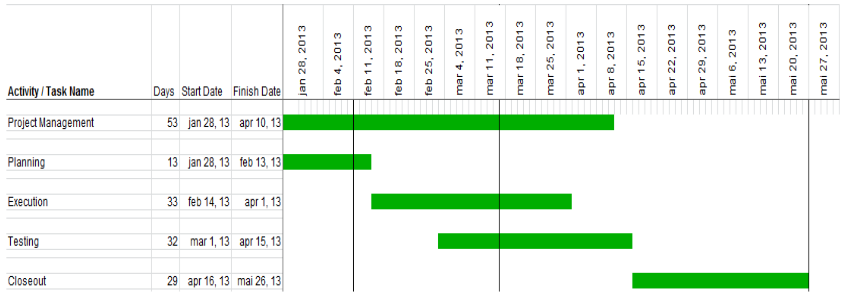
\includegraphics[scale=0.8]{images/gantt-diagram.png}
\caption{Gantt diagram. Milestones are marked using vertical lines}
\end{figure}

\section{Risk analysis}
The risk analysis states risks identified by the team. The importance of a risk is calculated by multiplying likelihood and impact. Higher number means higher importance for the project. 
\captionof{table}{Risk analysis}
\label{fig:risktable}
\begin{longtable}{|m{0.15 \textwidth}|m{0.1 \textwidth}|m{0.1 \textwidth}|m{0.1 \textwidth}|m{0.185 \textwidth}|m{0.185 \textwidth}|}
\hline
	\rowcolor{Gray}
	\textbf{Description} & \textbf{Likeli{-}hood} & \textbf{Impact} & \textbf{Impor{-}tance} & \textbf{Preventive\newline Action} & \textbf{Remedial\newline Action}\\
	\endfirsthead%
	\multicolumn{6}{l}%
	{{\bfseries Continued from previous page}} \\ \hline
	\rowcolor{Gray}
	\textbf{Description} & \textbf{Likeli{-}hood} & \textbf{Impact} & \textbf{Impor{-}tance} & \textbf{Preventive\newline Action} & \textbf{Remedial\newline Action}\\
\hline
	\endhead%
	\hline

	\hline \multicolumn{6}{|l|}{{Continued on next page}} \\ \hline
	\endfoot%

	\endlastfoot%

	Illness & 7 & 2 & 14 & Good\newline communication and effective use of GitHub & Increase workhours and exchange tasks and\newline responsibilities\\
\hline
	Project\newline complexity & 6 & 5 & 30 & Don't take on too much work & Cut down the demands\\
\hline
	Customer\newline issues & 1 & 5 & 5 & Agreement with customer and weekly feedback from customer & Use the\newline original\newline requirement specification\\
\hline
	License\newline incompability & 7 & 7 & 49 & Avoid\newline integrating components with incopatible licenses & Discover other implementations or implment from scratch\\
\hline
	Group\newline conflicts or disagreements & 3 & 3 & 9 & Keep close\newline contact to avoid\newline surprises.\newline Leader takes\newline action & Contact\newline supervisor and make an\newline appointment\\
\hline
	Over the air complexity & 8 & 8 & 64 & Have multiple\newline alternative\newline solutions and keep close\newline contact with customer & Detail what was attempted as well as why it couldn't be solved in the final report.\\
\hline
	Personal matters & 8 & 5 & 40 & Not much\newline preventative action can be taken & Keep in touch and stay\newline updated. In case you still can do tasks, claim one and tell the\newline others\\
\hline
\end{longtable}

\chapter{Requirements}
\subsection{Functional requirements}
\begin{table}[H]
\begin{tabularx}{\linewidth}{lX}
\textbf{FR01} & \textbf{Over the air installation}\\
 & The Android application and the Arduino device should communicate over bluetooth and install an arbitrary application from the Arduino Store in a simple two step process.\\
\textbf{FR02} & \textbf{Easy to use interface}\\
 & The Arduino Store application should be easy to use and easy to understand. It should not be necessary to do anything on the Arduino except for starting it. On startup it should search for nearby bluetooth connections with paired devices.\\
 \textbf{FR03} & \textbf{Example PUIs}\\
 & To demonstrate the Arduino Store (on Android), over the air installation, and the application in action on an Arduino.\\
\textbf{FR04} & \textbf{Validation of Arduino hardware and software}\\
 & The Android application should by default hide Arduino applications in the Arduino Store which are incompatible with the Arduino device depending on memory requirements and connected devices.\\
\end{tabularx}
\caption{Functional Requirements}
\end{table}

\subsection{Non-functional requirements}
\begin{table}[H]
\begin{tabularx}{\linewidth}{lX}
\textbf{NFR01} & \textbf{Usability}\\
 & Both old and young persons should be able to understand how to use the application and install arduino-apps.\\
\textbf{NFR02} & \textbf{Reliability}\\
 & The application on the Arduino should work and start if rebooted.\\
\textbf{NFR03} & \textbf{Open source}\\
 & The project is under European R\&D project SOCIETIES. All source code will be open source under Apache 2.0 license.\\
\textbf{NFR04} & \textbf{Platform compability}\\
 & Arduino Store should be compatible in Android 2.3 and newer. See FR04 for compatibility for Arduinos.\\
\textbf{NFR05} & \textbf{Extensibility}\\
 & It should be easy to add features and extend this product later. The system should therefore be modular to simplify further development.\\
\end{tabularx}
\caption{Non-functional requirements}
\end{table}
\chapter{Iterations}
\section{Iteration 1}
\begin{itemize}
	\item{Hold a concept demonstration for SINTEF (Powerpoint or role playing)}
	\begin{itemize}
		\item{Confirm understanding of the task}
		\item{Ideas for identifying the capabilities of an Arduino device and how to communicate these to the store client}
	\end{itemize}
	\item{Investigate potential solutions to faceilitate over the air installation of Arduino apps}
	\item{design the GUI for the app store}
\end{itemize}

\section{Iteration 2}
\begin{itemize}
	\item{Think architectural}
\end{itemize}
\chapter{Development environment}
\section{Development tools}
\subsection{Integrated Development Environments (IDEs)}
\subsubsection{Eclipse}
Eclipse is a freely available IDE implemented in Java. It has extensive plugin support and anyone can publish a plugin to support another programming language, versioning software or new program features alltogether. Eclipse provides useful, time saving functionality to developers, such as an extensive live debugging suite in addition to checking code syntax and providing auto completition of method calls.\\
Eclipse was chosen for Android development, due to previous experience with the software and good plugin support for targeting different versions of the Android API. Using a plugin for Arduino support was also considered, but the functionality of the available plugin was found lacking. %Ståle, kan du si mer her?

\paragraph{Mylyn plugins}
Mylin is a plugin meant to integrate with other plugins that provide access to task, issue and bug tracking repositories. Issues can be referenced or created quickly from the Eclipse IDE while coding, and the plugin can be configure to show relevant code sections when selecting an issue to work on. The group used a Github connector for Mylin to get Mylin to display and work with GitHub issues.

\paragraph{Android Software Development Kit (SDK)}
The Android SDK provides access to several versions of the Android API through the use of an installation manager. This allows for simple updating when new versions of the API are released, as well as supporting older devices. A simulator for testing against different Android devices is also available.

\subsubsection{Arduino IDE}
The Arduino IDE is provided by the creators of the Arduino platform as a free and open source program. It provides syntax checking, example programs, as well as basic editing tools. The IDE handles compilation of Arduino code into C and C++ code the regular microcontroller tools can handle (the IDE includes and depends on tools developed by Atmel, the company behind the chip Arduino uses) and can pass it on to an integrated uploading tool (avr-dude) to get it running on the Arduino.\\
The official Arduino IDE was considered for coding the Arduino component in, but due to its limited text and code related feature set (lacking features such as auto complete), the IDE was not used for coding.

\subsection{Codebase management and versioning}
\subsubsection{Git Version Control Software}
Git is a free, open source VCS with support for both local and remote repositories. It keeps track of differences between versions of files and allows for offline commits and branch creation, as this is done locally first before pushing the updates to a repository.\\
There are various terminal and front-end solutions available, including a GUI version from GitHub and Eclipse plugins. Past experiences with Git plugins for Eclipse led to a decision to use terminal software, as the GitHub program lacked advanced functionality regarding branching, among others. Another benefit with that solution was that the VCS then was IDE- and platform-independent and that there was no need to use the IDE for working with the report repository.
\subsubsection{GitHub}
Github hosts repositories for use with the Git VCS. They also provide basic issue tracking and social features, such as following other developers or projects. Paying customers can elect to hide their code, while free users have to share their code with everyone (one user can however keep one hidden project as long as he is the sole developer).\\
The customer required source code to be uploaded to Github and also recommended use of Github for requesting assistance using issues - a recommendation that was followed.\\

\section{Project management tools}
\subsection{Google Docs}
Google Docs is a free to use online office suite that allows users to simultaneously edit documents of different types (text, spreadsheet, presentation, et cetera), which was of great use when the group was working together on documents. It also supports document chat and comments (temporary chat/forum thread-like structure). Google Docs was used for editing the preliminary version of the report and other documents in connection with the project.

\subsection{Microsoft Word}
Microsoft Word is the de facto standard Word Processor, with support for many different effects (blinking letters, 3D text and so on). Content creation and formatting tasks are nearly completely intertwined, making it tricky to maintain a consistent document as the documents grow larger.\\
Microsoft Word was used to generate certain graphs for the preliminary reports.

\subsection{\LaTeX}
\LaTeX is a macro-improved version of Tex used for typesetting documents. It is free and open source. The general idea is to separate content creation and formatting to create consistent documents effectively without being distracted by the appearance of the content.\\
After the preliminary report, work on the report was written in \LaTeX.

\subsection{Google Calendar}
Google Calendar is a free to use online calendar. It supports both private and public events. Google Calendar allows for simple calendar synchronization across different devices and platforms.\\
A shared calendar in Google Calendar was created to make it easier to keep track of group meetings, meetings with the customer and so on.

\subsection{Dropbox}
Dropbox is a cross platform file synchronization and sharing service. Files in a specified folder are automatically kept in sync among different devices. It is also possible to share folders with other users and with the world at large (this will also serve HTML pages). The basic service is free, but comes with limited storage space.\\
Dropbox was used for sharing of various files within the group, such as compiled versions of the report, data sheets for Arduino components and so on. 

\subsection{Wunderlist}
Wunderlist is a free todo list tool supporting shared lists. It supports sharing tasks between the participants of a to-do list with reminders and notes.\\
Wunderlist was used to serve reminders for other, non-coding related tasks, like scheduling meetings or booking rooms.

\subsection{Doodle}
Doodle is a free online tool for scehduling events. It allows an user to create an event and aims to simplify scheduling of events by ''polling'' the participant when they are available. When the participants of the event has answered, one can easily view when all participants is available for meeting.\\
Doodle was used to schedule the first meetings the group had, before regular meetings were established. 
\chapter{Design and implentation}
The market app should be easy to use and fit for consumers of all ages. To install an application the user has to select a desired application with one touch, then check the specification if its compatible with the Arduino, then a agree/install button for installing the app on the Arduino. This is a total of two clicks, despite you have chosen a category or search hits on the market app. This is similar to Google Play.\\
\newline
Each (supported) Arduino device is equipped with a Unified Resource Identifier (URI) stored in its ROM. This URI is automatically transferred to the market app once it is turned on and is in range; the hardware configuration (Memory, connected devices) is stored in a XML file the URI links to.
The app store client can then compare compatibility with the device and app requirements.
Only apps supported on your Arduino will initially be visible in the market application, however, power users can enable unfiltered results to browse the selection and consider upgrading the device.\\
\newline
Anyone modifying a board will have to provide a hardware specification and transfer a new URI to the device if they want filtered results in the app store (Such a user could still choose to view and install unfiltered applications).
The URI could also be read from a QR-code.

\section{System Architecture}
	The design was divided into several modules:
	\begin{itemize}
		\item{Bluetooth connection between the Android and the Arduino}
		\item{Synchronization with the local SQLite database}
		\item{Android application view (the visible design)}
		\item{A service that contains the protocol for installing ``over the air''}
	\end{itemize}
	\vspace{0.2in}
	
	The system design was implemented such that further developing and extension should be as modular and easy as possible.
	Therefore it is designed as a plugin-like system where you easily can implement your own protocols against a desired device, e.g Raspberry Pi. The application only support STK500 protocol and therefore only connection towards Arduino.
	The design for the connection to other devices are done as following:\\

	\begin{figure}[H]
	\centering
	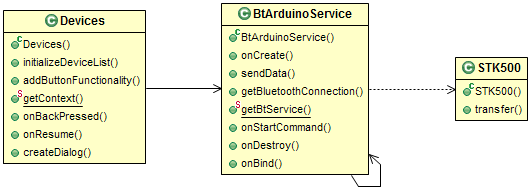
\includegraphics[width=130mm]{images/BTConnection.png}
	\end{figure}

	Devices.java is an Activity and can therefore be considered as a view in the application. To add a new service there is few changes to be done in Devices.java. Afterall an own service and a protocol towards a desired device must be implemented. Since this project only take in hand a connection between Android and Arduino, we implemented the STK500 protocol.
	The overall design solution for multiple connections will be like this:\\

	\begin{figure}[H]
	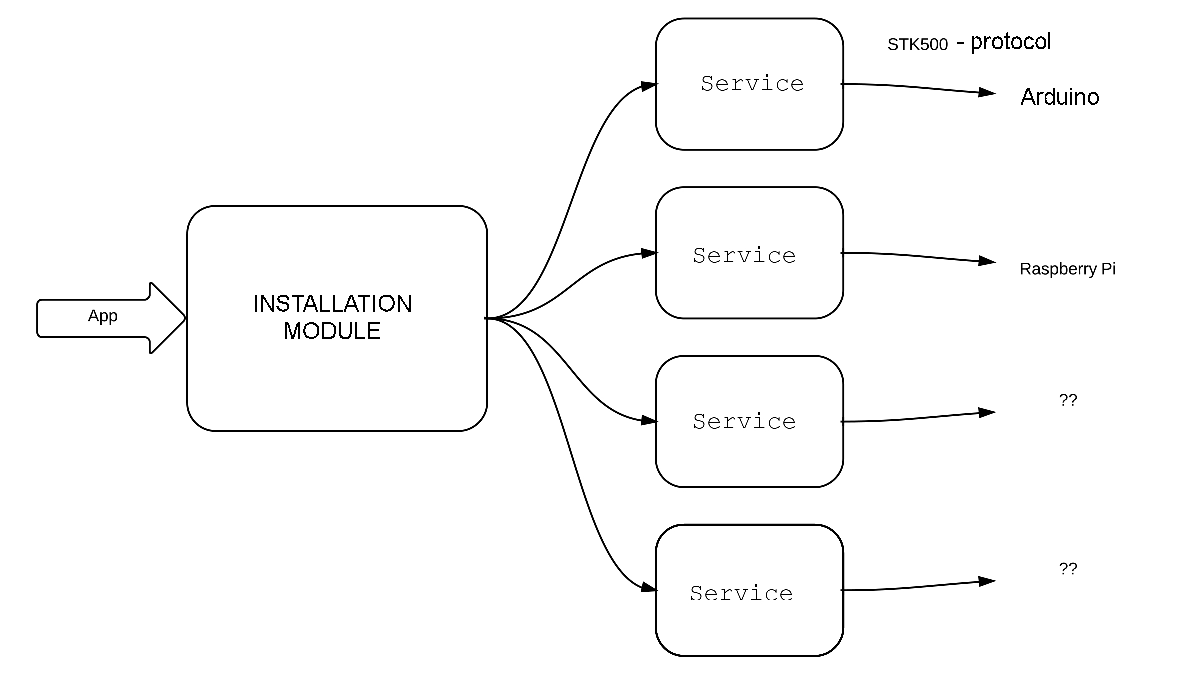
\includegraphics[scale=0.7]{figures/OTAArchitecture.pdf}
	\caption{Over The Air Architecture}
	\end{figure}

\section{Design of Android application}

%TODO Add short description about what the purpose of the application is?

Before the programming of the Android application was started, a complete design guide were created. In this section we have presented the complete design of the application. This guide were made for two reasons:
\begin{itemize}
	\item{Presentation for the customer.} With a complete design guide it was possible to present the user interface of the application to the customer before it was programmed. This allowed for input from the customer at a early stage, when it was easy to change the design.
	\item{Avoid confusion.} A design guide reduce the amount of confusion and discussion regarding the appearance of the user interface. When the looks of the user interface is settled before the programming is started, there is no need to discuss this along the way. 
\end{itemize}

\subsection{Design guide}
Following is the complete design guide of the Android application. Minor changes were made to some of the screens. In these cases it is commented below the picture. The design of the preferences screen is not showed, as it was unnecessary to design this screen.

\paragraph{Screen 1a - Device list}
Screen that shows the list of available Arduino devices. In the final design the list of devices fills the whole screen, and the buttons and description text has switched places. When a device is clicked, a progress bar appears and stays on the screen until a valid bluetooth connection with the chosen device is made.

\begin{figure}[H]
\centering
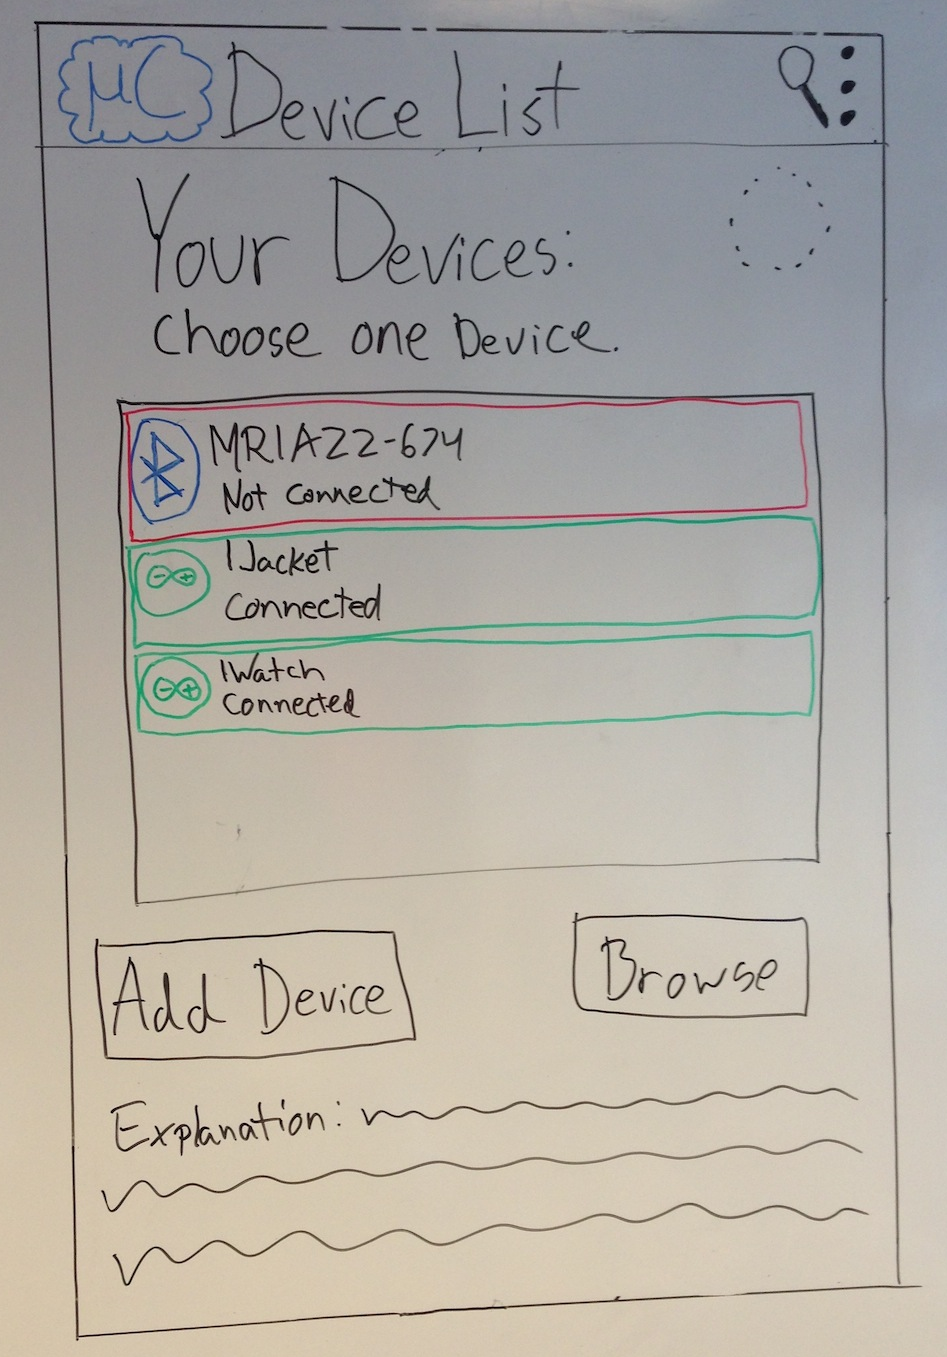
\includegraphics[scale=0.2]{images/Design_guide/Screen1a.png}
\caption{Screen 1a - Device list}
\end{figure}


\paragraph{Screen 1b - Add device manually}
Screen that appears after pressing the ''Add device'' button in Screen 1a. It was chosen to remove the ''Bluetooth settings'' button, as it unnecessary. In the final design, this screen contains only the ''QR code'' button and ''Input serial'' button, with a short description of the functionality of the button between them.

\begin{figure}[H]
\centering
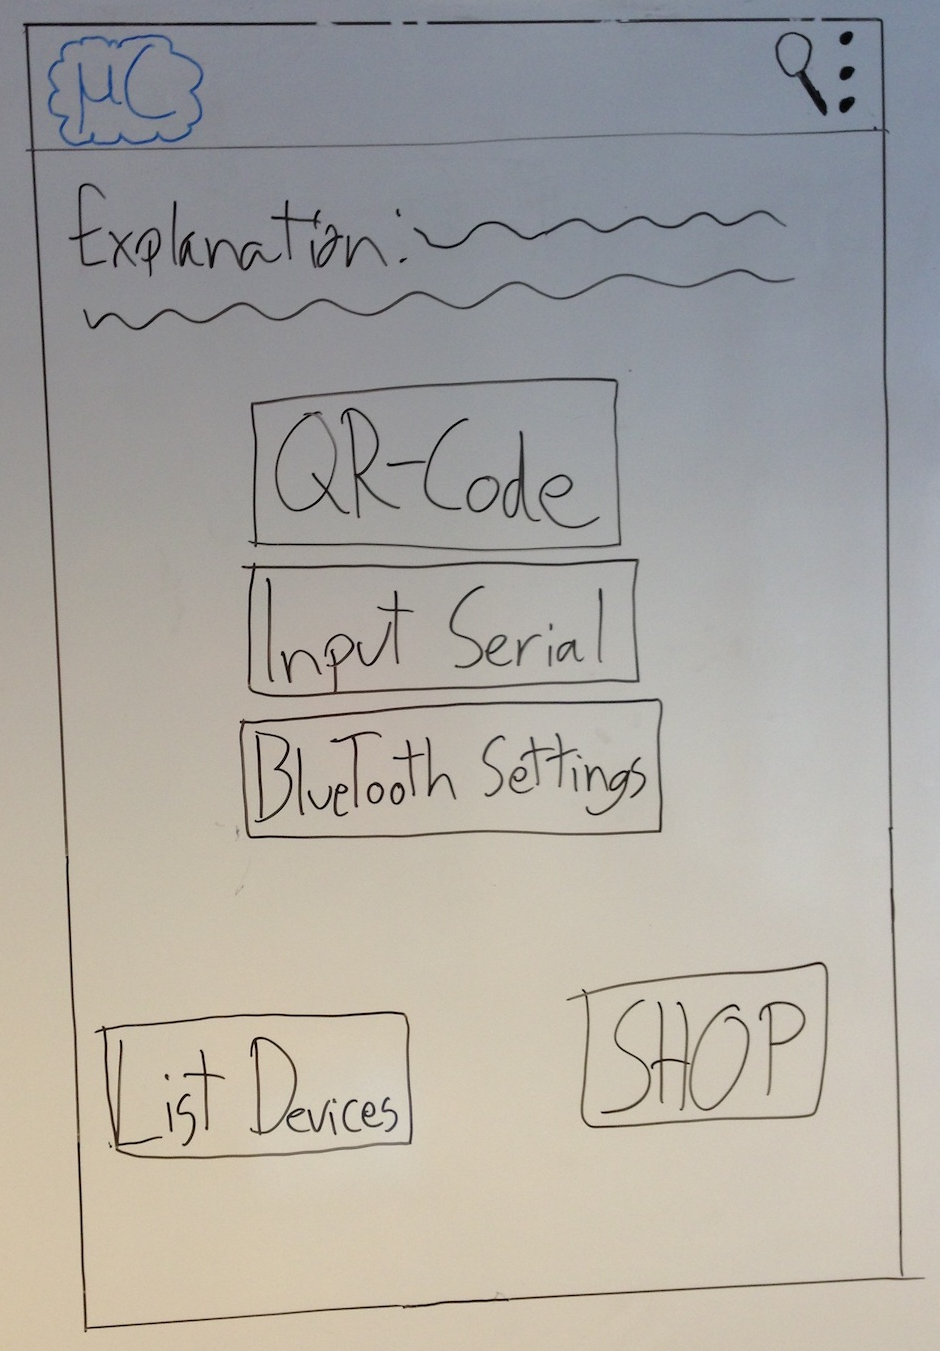
\includegraphics[scale=0.2]{images/Design_guide/Screen1b.png}
\caption{Screen 1b - Add device manually}
\end{figure}


\paragraph{Screen 1b-i - Input serial}
%Link to Screen 1b-i
Screen that appears when the ''Input serial'' button is clicked.

\begin{figure}[H]
\centering
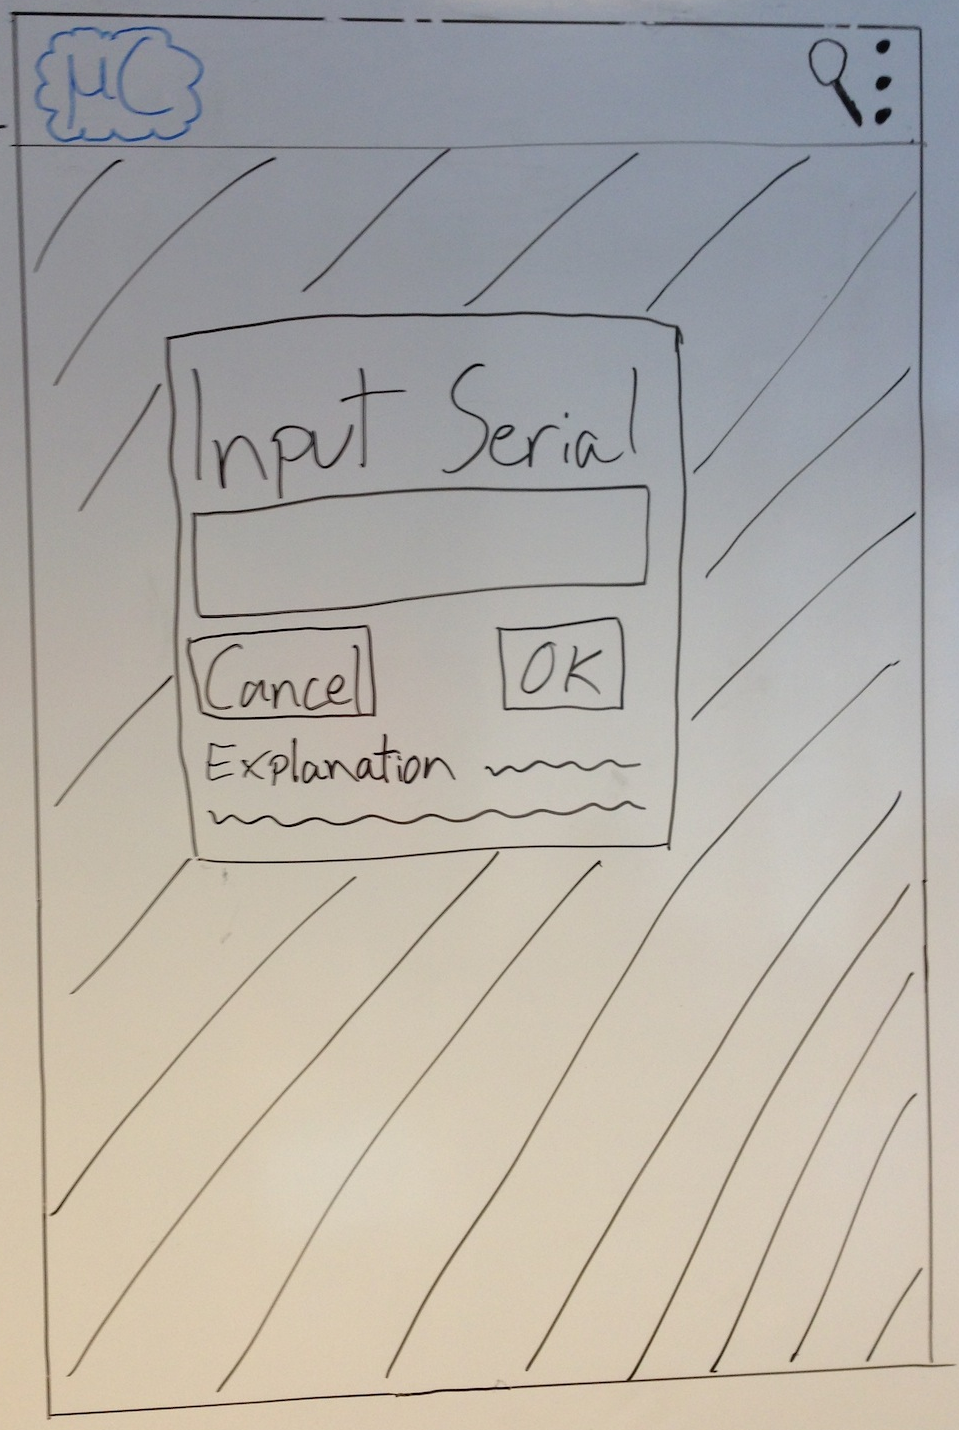
\includegraphics[scale=0.2]{images/Design_guide/Screen1b-i.png}
\caption{Screen 1b-i - Input serial}
\end{figure}


\paragraph{Screen 2a - Browse shop}
%Link to Screen 2a
Screen for browsing all the applications for Arduino in the shop. More categories have been added. The user can here swipe left/right to sort the available applications in different ways. See next paragraph.

\begin{figure}[H]
\centering
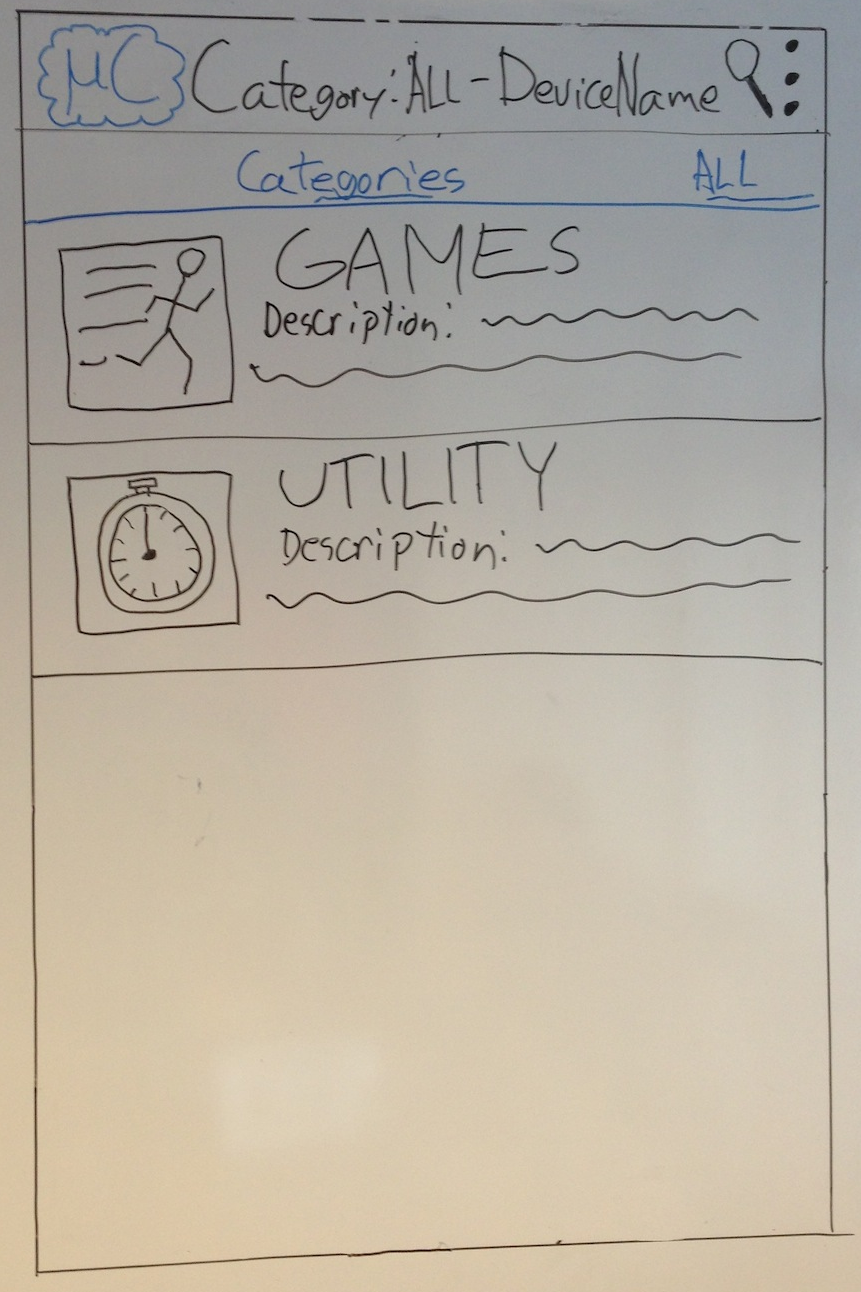
\includegraphics[scale=0.2]{images/Design_guide/Screen2a.png}
\caption{Screen 2a - Browse shop}
\end{figure}


\paragraph{Screen 2b - Browse shop by category}
%Link to Screen 2b
Screen that shows a list of all applications in chosen category. Category ''All'' is chosen.

\begin{figure}[H]
\centering
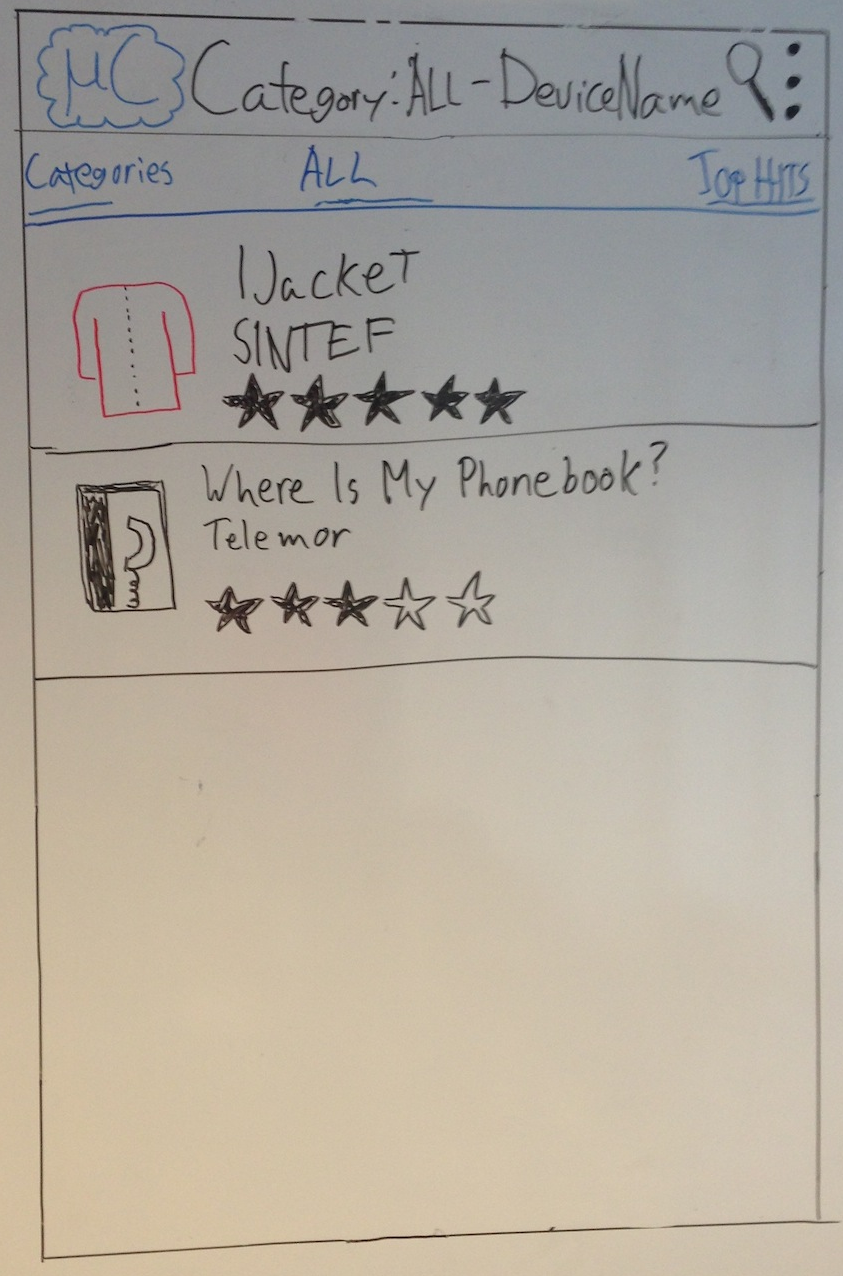
\includegraphics[scale=0.2]{images/Design_guide/Screen2b.png}
\caption{Screen 2b - Browse shop by category}
\end{figure}


\paragraph{Screen 3a - Application view}
%Link to Screen 3a
Screen with overview of an chosen application. Small changes were as comments field and reviews were given a lower priority at mid-term. 

\begin{figure}[H]
\centering
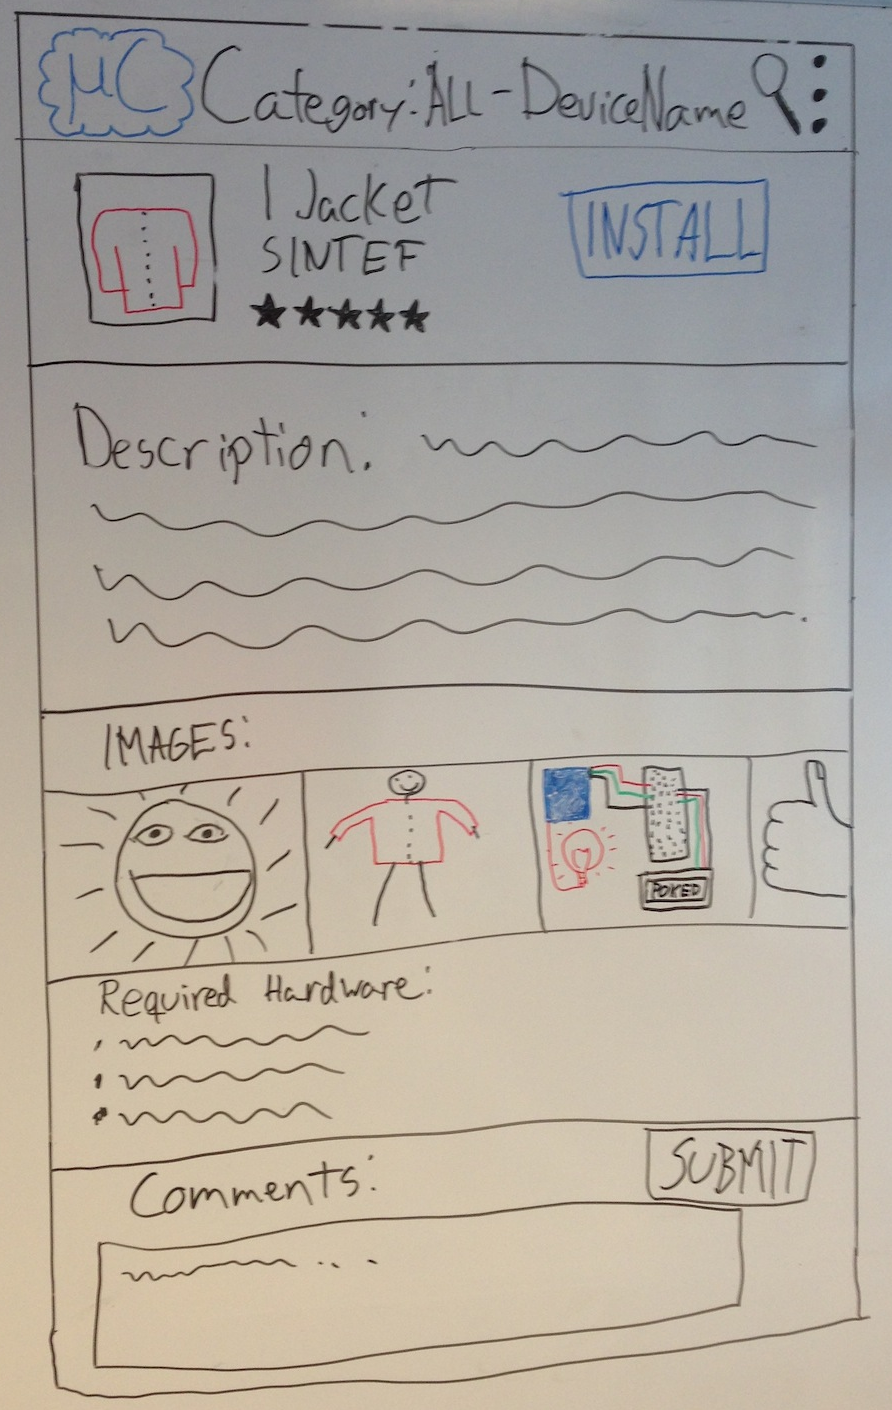
\includegraphics[scale=0.2]{images/Design_guide/Screen3a.png}
\caption{Screen 3a - Application view}
\end{figure}


\paragraph{Screen 3a-i - Installation confirmation}
%Link to Screen 3a-i
Screen that appears when the ''Install'' button in Screen 3a is pressed. Shows the name of the chosen device.

\begin{figure}[H]
\centering
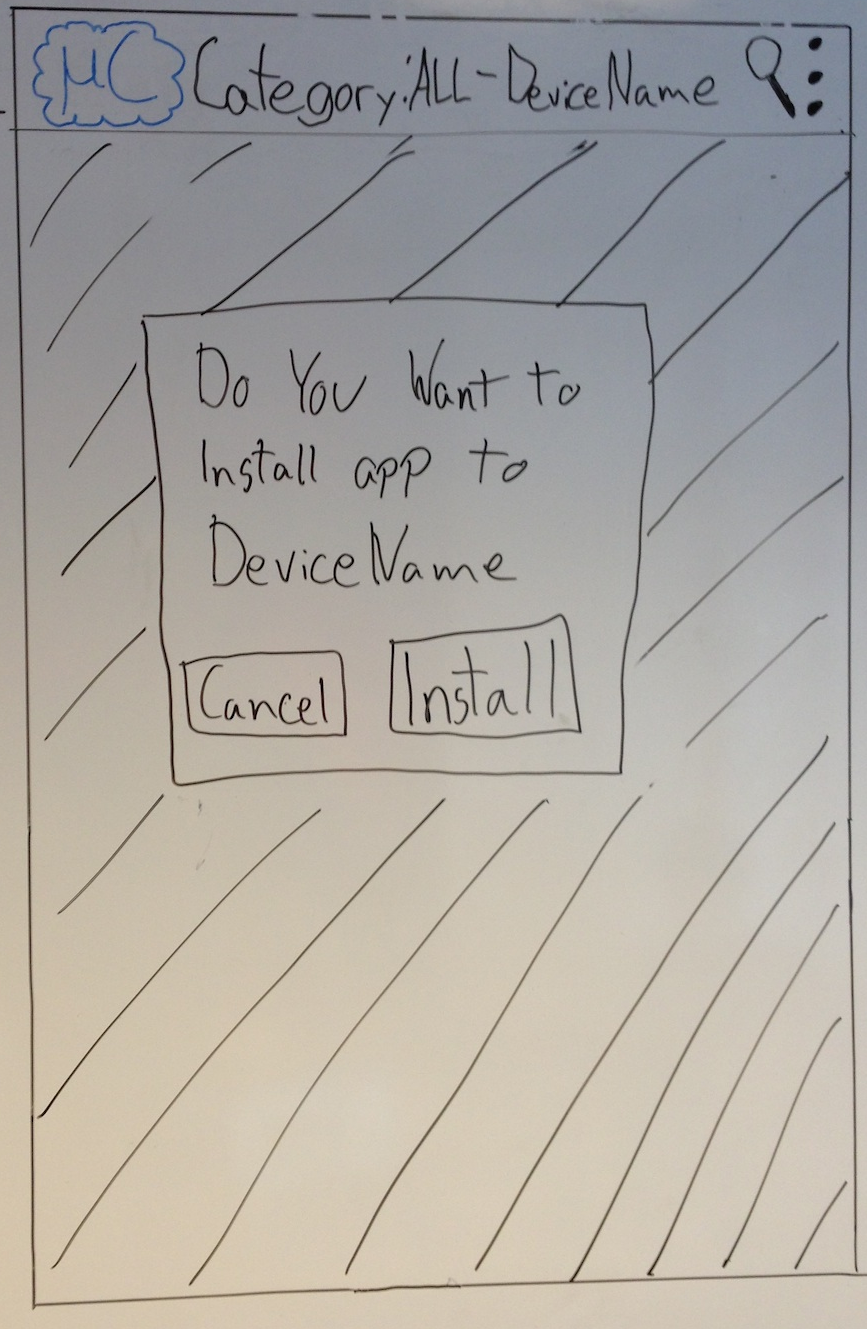
\includegraphics[scale=0.2]{images/Design_guide/Screen3a-i.png}
\caption{Screen 3a-i - Installation confirmation}
\end{figure}


\paragraph{Screen 3a-ii - Progress of installation}
%Link to Screen 3a-ii
Screen that shows the progress of the installation. The progress bar cannot be dismissed, so the Android application is locked until the installation is complete or has failed. 

\begin{figure}[H]
\centering
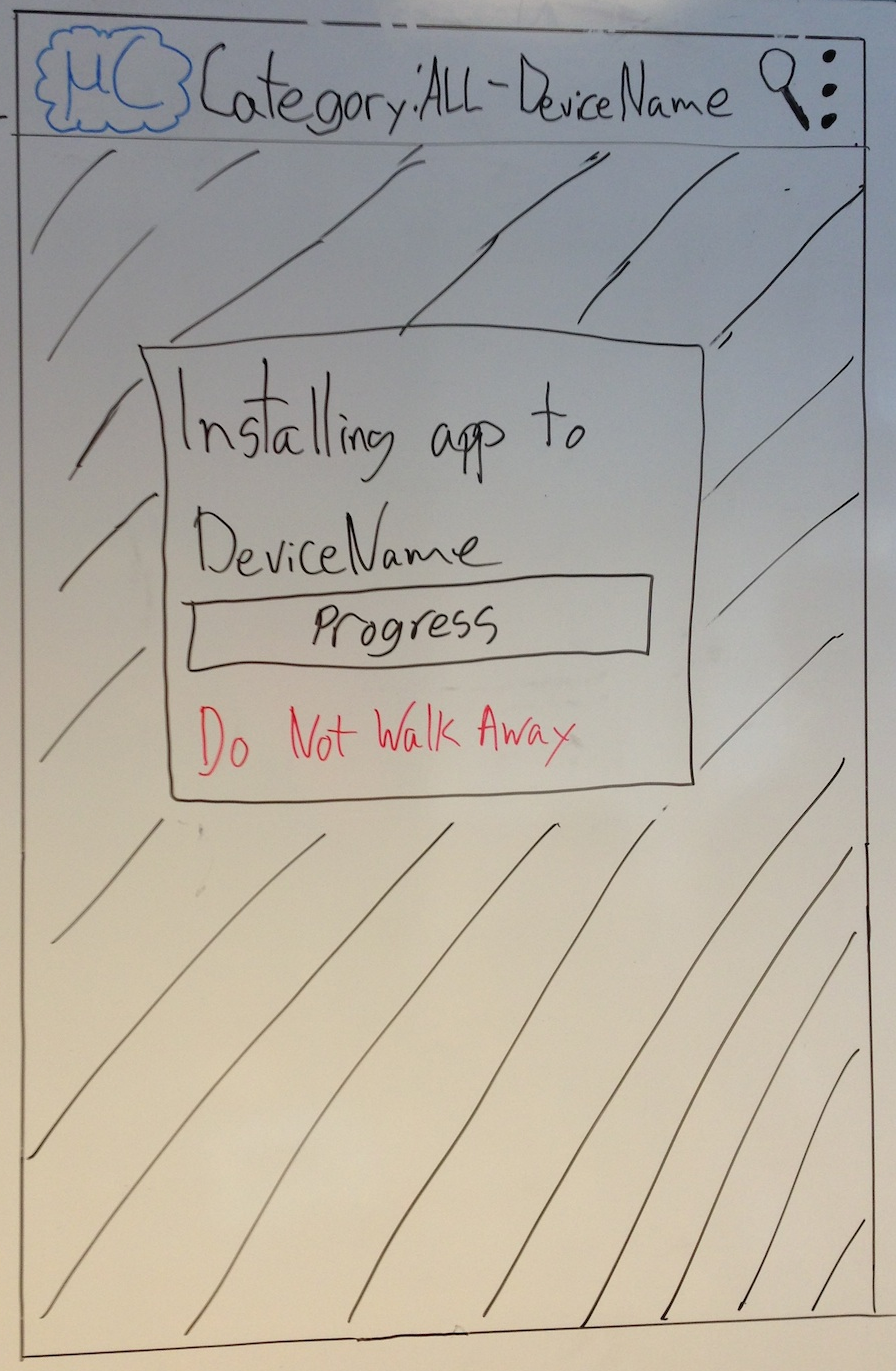
\includegraphics[scale=0.2]{images/Design_guide/Screen3a-ii.png}
\caption{Screen 3a-ii - Progress of installation}
\end{figure}


\paragraph{Screen Xa - Action overflow}
%Link to Screen Xa
Screen that appears when the ''Action overflow'' button is clicked. This menu is available from all the screen in the application with the exception of the preferences screen.

\begin{figure}[H]
\centering
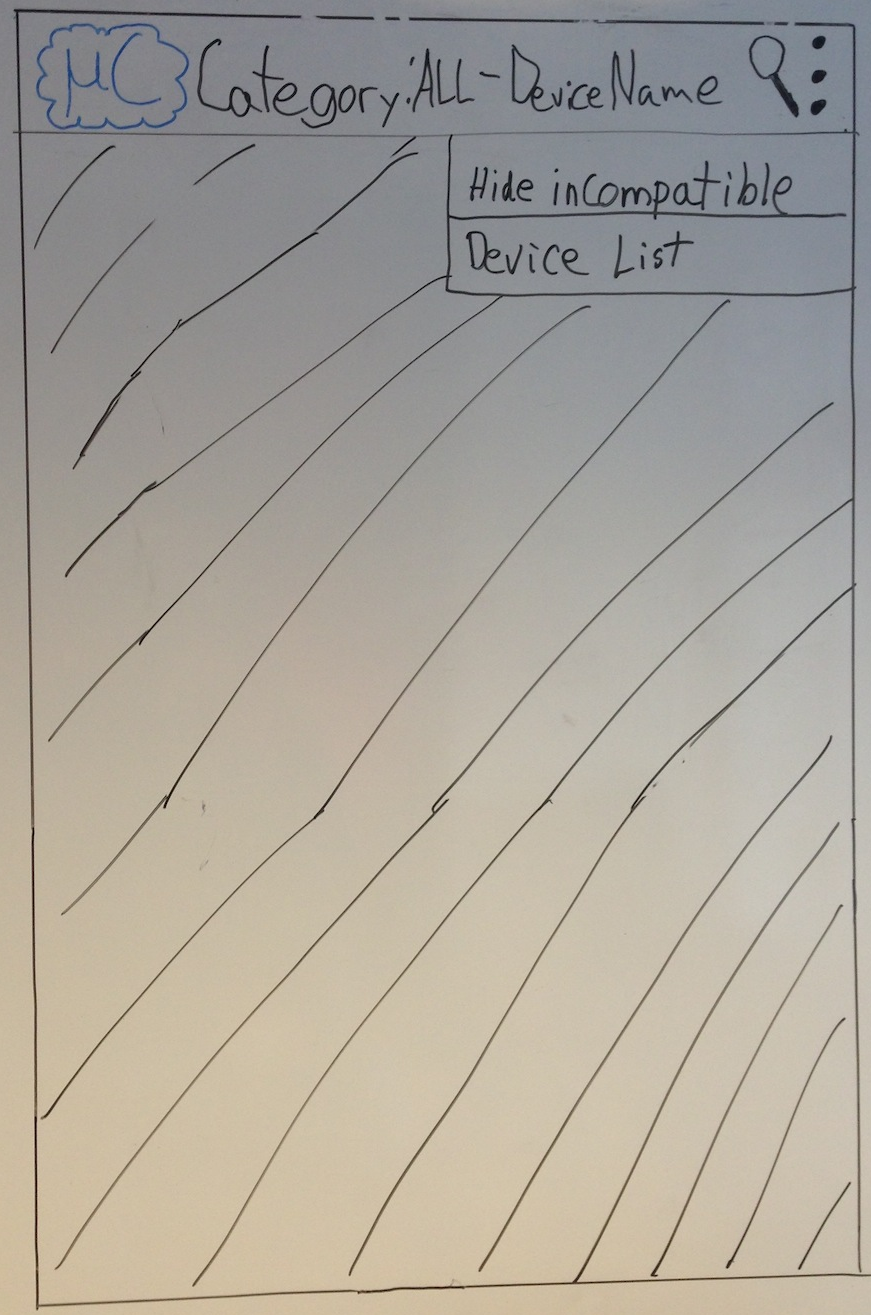
\includegraphics[scale=0.2]{images/Design_guide/ScreenXa.png}
\caption{Screen Xa - Action overflow}
\end{figure}

\section{Testing}
\ldots
%\section{Evalutation}
\subsection{Team roles}
The group was organized in different roles based on skill and experience. Each team member was given a responsibility for some code-packages. Further, the team was divided in six subgroups where each subgroup had one responsible leader. These were respectively group leader, documentation and substitute leader, arduino and PUI, Android and GUI, and test leader.

\subsubsection{Role evaluation}
The division of the group was an important feature. Every member knew who to contact about a specific problem, and who to contact regarding different tasks.
\begin{description}
	\item[Group leader]{The group leader was responsible the progress in the overall project. He ensured progress and priorities for deadlines.}
	\item[Documentation and subsitute leader]{Responsible for management of documentation and reports. In absence of the group leader, this role took on the group leaders responsibilities. This role were also responsible for contact with the customer and supervisor. }
	\item[Arduino and PUI]{Was responsible for the arduino part of the project. This implies contacting the arduino-lab, requirements of hardware, the coding part and over-the-air installation. This role were also responsible for development of the PUI examples.
}
	\item[Android and GUI]{Was responsible for the arduino part of the project. This implies contacting the arduino-lab, requirements of hardware, the coding part and over-the-air installation. This role were also responsible for development of the PUI examples.
}
	\item[Test leader]{The test leader were responsible for developing and executing test for the complete project.}
\end{description}
\begin{table}
\begin{tabular}{|l|l|}
\hline
	{\bf Name} & {\bf Role}\\
\hline
	Jeppe Benterud Eriksen & Group leader\\
\hline
	Nina Margrethe Smørsgård & Documantation and subsititue leader\\
\hline
	Robin Tordly & Android and GUI leader\\
\hline
	Bjørn Arve Fossum & PUI and Arduino leader\\
\hline
	Ståle Semb Hauknes & \emph{Over the Air} leader\\
\hline
	Wilhelm Walberg Schive & Test Leader\\
\hline
\end{tabular}
\caption{Roles}
\end{table}

\subsection{Existing solutions}
This is a summary of existing solutions similar to the project assignment. This section is divided in two subsections; one for the market application and one for the over-the-air transfer. The existing products were evaluated on the following criteria:
\begin{itemize}
	\item{To what degree the product fits the assignment.}
	\item{Can the product, or parts of it, be reused for the assignment? Can it lead to licensing issues?}
\end{itemize}

\subsubsection{Market application}
A prior project created an universal app store in PHP. Had potential for serving as a back end.

{\bf Google Play} is a similar market application for android that categorizes the applications and have a search option. It also knows what model of phone that is being used, and only show apps that is supported by that phone. The applications are shown in lists and can be downloaded by two clicks. The first click guides you to a description section with pictures, description, comments and user-feedback in form of 5-star-rating.\\
The store is not open source and can only be a source of inspiration for this project.
\begin{figure}[H]
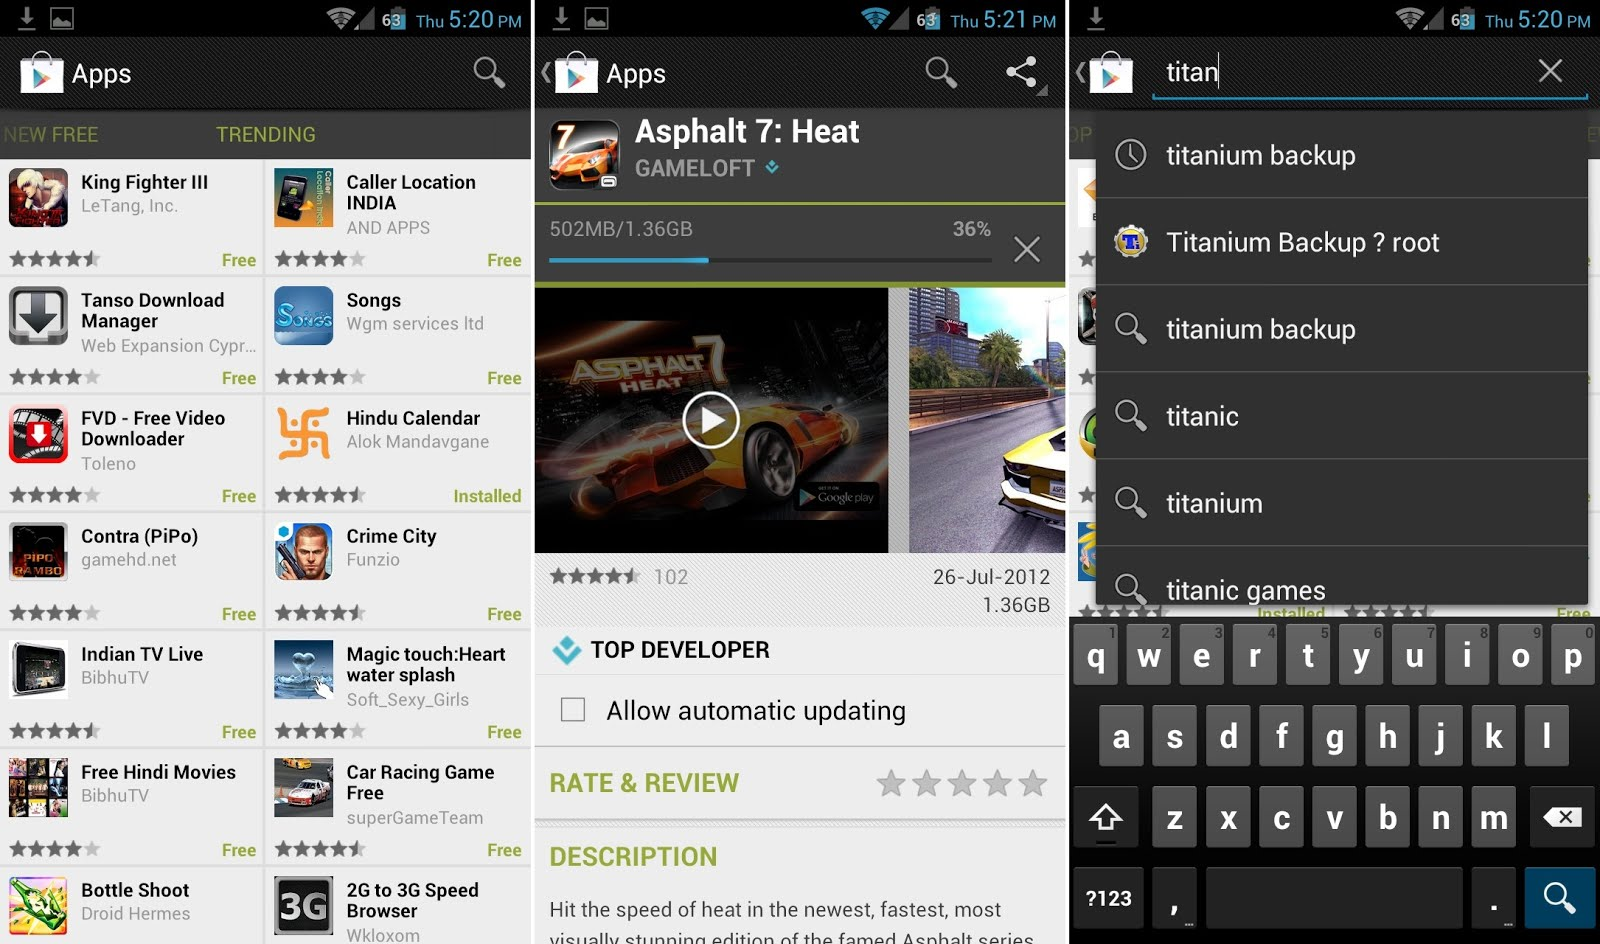
\includegraphics[scale=0.2]{images/Google-Play-Store-APK-3-7-15.jpg}
\caption{Google Play Store}
\end{figure}

{\bf App Store} is also a similar market application, but for apple products\ldots etc\ldots\\
\begin{figure}[H]
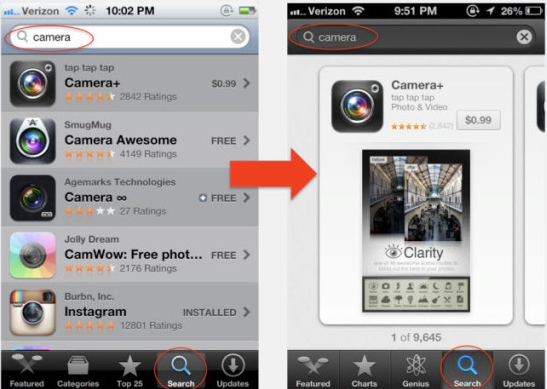
\includegraphics[scale=0.7]{images/png;base642dee0c596030bc1e.png}
\caption{App Store}
\end{figure}
These applications fit the assignment in the way that they are both market applications where one can download applications. This were useful for the development of the product, since it was possible to use the same principles in the assignment. It is also similar in the way that it is possible to browse for applications on the computer, and ''push'' the app to a mobile telephone. This, however, does not connect via bluetooth which the task assignment stated that the finished product should. Based on this, it was not possible to reuse the code or other parts of any of the applications in the development. 

\subsubsection{Over the air transfer}
Pebble is a watch that offers over the air transfer of applications. It is based on the same microchip as one of the newest Arduino\#, but contains an operating system written in C.
\begin{figure}[H]
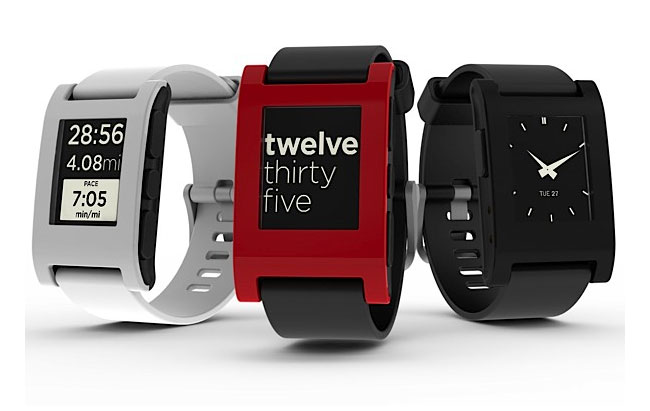
\includegraphics[scale=0.7]{images/Pebble-Smartphone-Watch.jpeg}
\caption{Pebble Watch}
\end{figure}
There is very little documentation on the Pebble website, so the potential reuse in this project appears minimal. %TODO Rename chapter to Reflection

\newpage
\addcontentsline{toc}{section}{Appendixes} %this line may break your compilation, and may require recompiation
\appendix
%\input{section/}

\newpage
\listoftables
\listoffigures
\bibliographystyle{plain}


% We use MLA standard for citation. Create your citations at:
% http://citationmachine.net/index2.php?reqstyleid=0&stylebox=1

\begin{thebibliography}{9}

	\bibitem{scrum}{
		\emph{Scrum.org}.
		N.p.. Web. 13 Mar 2013
		<http://www.scrum.org/Resources/What-is-Scrum>.
		}

	%Citation for 'software engineering'
	\bibitem{sommerville}{
		Sommerville, Ian. \emph{Software Engineering}. 9th ed. Boston: Pearson Custom Publishing, 2011. Print.
	  	}

    \bibitem{poppendieck}{
        Poppendieck, M., and T. Poppendieck. \emph{Lean software development, an agile toolkit}. Addison-Wesley Professional, 2003. Print.
        }

    \bibitem{integration-testing1}{
    	\emph{Wikipedia.org}
    	<http://en.wikipedia.org/wiki/Integration\_testing>
    }

    \bibitem{integration-testing2}{
		\emph{Microsoft.com}
		<http://msdn.microsoft.com/en-us/library/aa292128(v=vs.71).aspx>
	}
	
	\bibitem{functional-testing}{
		\emph{Wikipedia.org}
		<http://en.wikipedia.org/wiki/Functional\_testing>
	}
	
	\bibitem{unit-testing1}{
		\emph{Microsoft.com}
		<http://msdn.microsoft.com/en-us/library/aa292197(v=vs.71).aspx>
	}
	
	\bibitem{unit-testing2}{
		\emph{Wikipedia.org}
		<http://en.wikipedia.org/wiki/Unit\_testing>
	}
	
	\bibitem{unit-testing3}{
		\emph{Android.com}
		<http://developer.android.com/tools/testing/testing\_android.html>
	}
	
	\bibitem{testing-overview}{
		\emph{Microsoft.com}
		<http://msdn.microsoft.com/en-us/library/aa292191(v=vs.71).aspx>
	}
	
	\bibitem{validation-testing1}{
		\emph{Wikipedia.org}
		<http://en.wikipedia.org/wiki/Verification\_and\_validation>
	}
	
	\bibitem{validation-testing2}{
		\emph{Buzzle.com}
		<http://www.buzzle.com/articles/validation-testing.html>
	}

    \bititem{kruchten}{
        Kroll, P., and P. Kruchten. \emph{The rational unified process made easy: A practitioner\'s guide to the rup}. Boston, MA: Addison-Wesley Professional, 2003. eBook.
        }

\end{thebibliography}


\end{document}
